\documentclass{standalone}
\usepackage{tikz}
\usetikzlibrary{patterns, positioning}


\begin{document}
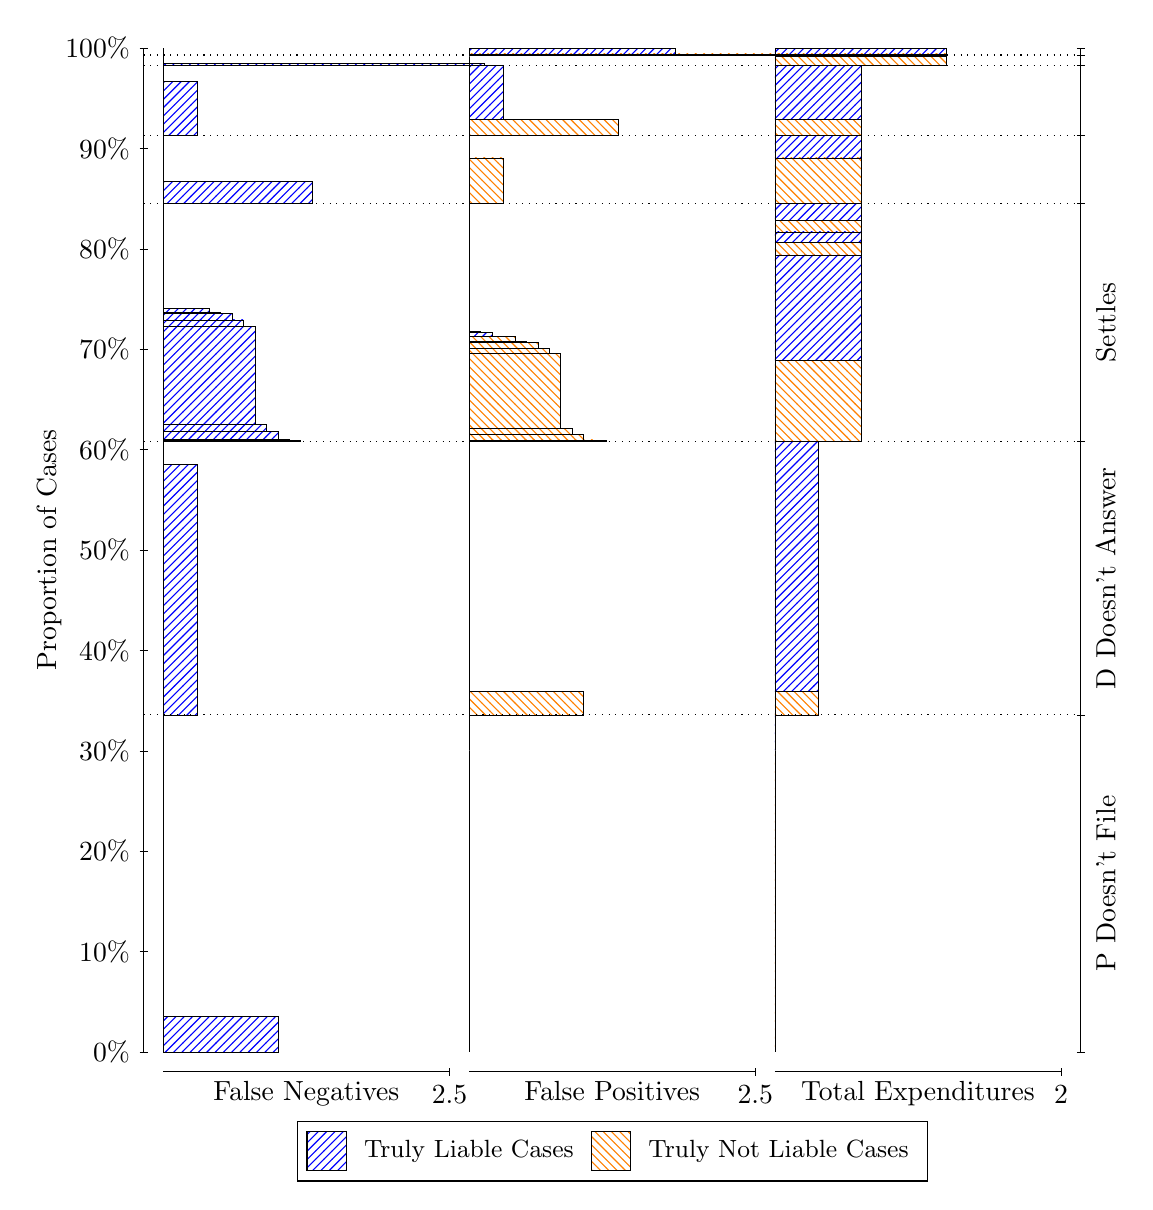
\begin{tikzpicture}
\draw[black, very thin] (1.5,1.75) -- (1.5,14.5);
\node[rotate=90, text=black, anchor=center] at (0.3, 8.125) {Proportion of Cases};
\draw[black, very thin] (1.45,1.75) -- (1.55,1.75);
\node[text=black, anchor=east] at (1.45, 1.75) {0\%};
\draw[black, very thin] (1.45,3.025) -- (1.55,3.025);
\node[text=black, anchor=east] at (1.45, 3.025) {10\%};
\draw[black, very thin] (1.45,4.3) -- (1.55,4.3);
\node[text=black, anchor=east] at (1.45, 4.3) {20\%};
\draw[black, very thin] (1.45,5.575) -- (1.55,5.575);
\node[text=black, anchor=east] at (1.45, 5.575) {30\%};
\draw[black, very thin] (1.45,6.85) -- (1.55,6.85);
\node[text=black, anchor=east] at (1.45, 6.85) {40\%};
\draw[black, very thin] (1.45,8.125) -- (1.55,8.125);
\node[text=black, anchor=east] at (1.45, 8.125) {50\%};
\draw[black, very thin] (1.45,9.4) -- (1.55,9.4);
\node[text=black, anchor=east] at (1.45, 9.4) {60\%};
\draw[black, very thin] (1.45,10.675) -- (1.55,10.675);
\node[text=black, anchor=east] at (1.45, 10.675) {70\%};
\draw[black, very thin] (1.45,11.95) -- (1.55,11.95);
\node[text=black, anchor=east] at (1.45, 11.95) {80\%};
\draw[black, very thin] (1.45,13.225) -- (1.55,13.225);
\node[text=black, anchor=east] at (1.45, 13.225) {90\%};
\draw[black, very thin] (1.45,14.5) -- (1.55,14.5);
\node[text=black, anchor=east] at (1.45, 14.5) {100\%};

\draw[black, very thin] (13.4,1.75) -- (13.4,14.5);
\draw[black, very thin] (13.35,1.75) -- (13.45,1.75);
\node[anchor=west] at (13.35, 1.75) {};
\draw[black, very thin] (13.35,6.0313) -- (13.45,6.0313);
\node[anchor=west] at (13.35, 6.0313) {};
\draw[black, very thin] (13.35,9.5049) -- (13.45,9.5049);
\node[anchor=west] at (13.35, 9.5049) {};
\draw[black, very thin] (13.35,12.525) -- (13.45,12.525);
\node[anchor=west] at (13.35, 12.525) {};
\draw[black, very thin] (13.35,13.386) -- (13.45,13.386);
\node[anchor=west] at (13.35, 13.386) {};
\draw[black, very thin] (13.35,14.282) -- (13.45,14.282);
\node[anchor=west] at (13.35, 14.282) {};
\draw[black, very thin] (13.35,14.412) -- (13.45,14.412);
\node[anchor=west] at (13.35, 14.412) {};
\draw[black, very thin] (13.35,14.5) -- (13.45,14.5);
\node[anchor=west] at (13.35, 14.5) {};

\draw[black, very thin, pattern color=blue, pattern=north east lines] (1.75,1.75) rectangle (3.2033,2.2002);
\draw[black, very thin, pattern color=orange, pattern=north west lines] (1.75,2.2002) rectangle (1.75,6.0313);
\draw[black, very thin, pattern color=blue, pattern=north east lines] (1.75,6.0313) rectangle (2.186,9.2089);
\draw[black, very thin, pattern color=orange, pattern=north west lines] (1.75,9.2089) rectangle (1.75,9.5049);
\draw[black, very thin, pattern color=blue, pattern=north east lines] (1.75,9.5049) rectangle (3.494,9.5211);
\draw[black, very thin, pattern color=blue, pattern=north east lines] (1.75,9.5211) rectangle (3.3487,9.5307);
\draw[black, very thin, pattern color=blue, pattern=north east lines] (1.75,9.5307) rectangle (3.2033,9.6275);
\draw[black, very thin, pattern color=blue, pattern=north east lines] (1.75,9.6275) rectangle (3.058,9.6346);
\draw[black, very thin, pattern color=blue, pattern=north east lines] (1.75,9.6346) rectangle (3.058,9.7243);
\draw[black, very thin, pattern color=blue, pattern=north east lines] (1.75,9.7243) rectangle (2.9127,10.967);
\draw[black, very thin, pattern color=blue, pattern=north east lines] (1.75,10.967) rectangle (2.7673,11.047);
\draw[black, very thin, pattern color=blue, pattern=north east lines] (1.75,11.047) rectangle (2.622,11.132);
\draw[black, very thin, pattern color=blue, pattern=north east lines] (1.75,11.132) rectangle (2.4767,11.142);
\draw[black, very thin, pattern color=blue, pattern=north east lines] (1.75,11.142) rectangle (2.3313,11.19);
\draw[black, very thin, pattern color=orange, pattern=north west lines] (1.75,11.19) rectangle (1.75,12.525);
\draw[black, very thin, pattern color=blue, pattern=north east lines] (1.75,12.525) rectangle (3.6393,12.807);
\draw[black, very thin, pattern color=orange, pattern=north west lines] (1.75,12.807) rectangle (1.75,13.386);
\draw[black, very thin, pattern color=blue, pattern=north east lines] (1.75,13.386) rectangle (2.186,14.072);
\draw[black, very thin, pattern color=orange, pattern=north west lines] (1.75,14.072) rectangle (1.75,14.282);
\draw[black, very thin, pattern color=blue, pattern=north east lines] (1.75,14.282) rectangle (5.8193,14.3);
\draw[black, very thin, pattern color=orange, pattern=north west lines] (1.75,14.3) rectangle (1.75,14.412);
\draw[black, very thin, pattern color=orange, pattern=north west lines] (1.75,14.412) rectangle (1.75,14.425);
\draw[black, very thin, pattern color=blue, pattern=north east lines] (1.75,14.425) rectangle (1.75,14.5);
\draw[black, very thin, pattern color=orange, pattern=north west lines] (5.6333,1.75) rectangle (5.6333,5.5811);
\draw[black, very thin, pattern color=blue, pattern=north east lines] (5.6333,5.5811) rectangle (5.6333,6.0313);
\draw[black, very thin, pattern color=orange, pattern=north west lines] (5.6333,6.0313) rectangle (7.0867,6.3272);
\draw[black, very thin, pattern color=blue, pattern=north east lines] (5.6333,6.3272) rectangle (5.6333,9.5049);
\draw[black, very thin, pattern color=orange, pattern=north west lines] (5.6333,9.5049) rectangle (7.3773,9.5166);
\draw[black, very thin, pattern color=orange, pattern=north west lines] (5.6333,9.5166) rectangle (7.232,9.5248);
\draw[black, very thin, pattern color=orange, pattern=north west lines] (5.6333,9.5248) rectangle (7.0867,9.5975);
\draw[black, very thin, pattern color=orange, pattern=north west lines] (5.6333,9.5975) rectangle (6.9413,9.6682);
\draw[black, very thin, pattern color=orange, pattern=north west lines] (5.6333,9.6682) rectangle (6.796,10.618);
\draw[black, very thin, pattern color=orange, pattern=north west lines] (5.6333,10.618) rectangle (6.6507,10.685);
\draw[black, very thin, pattern color=orange, pattern=north west lines] (5.6333,10.685) rectangle (6.5053,10.759);
\draw[black, very thin, pattern color=orange, pattern=north west lines] (5.6333,10.759) rectangle (6.36,10.774);
\draw[black, very thin, pattern color=orange, pattern=north west lines] (5.6333,10.774) rectangle (6.2147,10.84);
\draw[black, very thin, pattern color=blue, pattern=north east lines] (5.6333,10.84) rectangle (5.924,10.887);
\draw[black, very thin, pattern color=blue, pattern=north east lines] (5.6333,10.887) rectangle (5.7787,10.898);
\draw[black, very thin, pattern color=blue, pattern=north east lines] (5.6333,10.898) rectangle (5.6333,12.525);
\draw[black, very thin, pattern color=orange, pattern=north west lines] (5.6333,12.525) rectangle (6.0693,13.104);
\draw[black, very thin, pattern color=blue, pattern=north east lines] (5.6333,13.104) rectangle (5.6333,13.386);
\draw[black, very thin, pattern color=orange, pattern=north west lines] (5.6333,13.386) rectangle (7.5227,13.596);
\draw[black, very thin, pattern color=blue, pattern=north east lines] (5.6333,13.596) rectangle (6.0693,14.282);
\draw[black, very thin, pattern color=orange, pattern=north west lines] (5.6333,14.282) rectangle (5.6333,14.394);
\draw[black, very thin, pattern color=blue, pattern=north east lines] (5.6333,14.394) rectangle (5.6333,14.412);
\draw[black, very thin, pattern color=orange, pattern=north west lines] (5.6333,14.412) rectangle (9.7027,14.425);
\draw[black, very thin, pattern color=blue, pattern=north east lines] (5.6333,14.425) rectangle (8.2493,14.5);
\draw[black, very thin, pattern color=orange, pattern=north west lines] (9.5167,1.75) rectangle (9.5167,5.5811);
\draw[black, very thin, pattern color=blue, pattern=north east lines] (9.5167,5.5811) rectangle (9.5167,6.0313);
\draw[black, very thin, pattern color=orange, pattern=north west lines] (9.5167,6.0313) rectangle (10.062,6.3272);
\draw[black, very thin, pattern color=blue, pattern=north east lines] (9.5167,6.3272) rectangle (10.062,9.5049);
\draw[black, very thin, pattern color=orange, pattern=north west lines] (9.5167,9.5049) rectangle (10.607,10.535);
\draw[black, very thin, pattern color=blue, pattern=north east lines] (9.5167,10.535) rectangle (10.607,11.873);
\draw[black, very thin, pattern color=orange, pattern=north west lines] (9.5167,11.873) rectangle (10.607,12.035);
\draw[black, very thin, pattern color=blue, pattern=north east lines] (9.5167,12.035) rectangle (10.607,12.164);
\draw[black, very thin, pattern color=orange, pattern=north west lines] (9.5167,12.164) rectangle (10.607,12.307);
\draw[black, very thin, pattern color=blue, pattern=north east lines] (9.5167,12.307) rectangle (10.607,12.525);
\draw[black, very thin, pattern color=orange, pattern=north west lines] (9.5167,12.525) rectangle (10.607,13.104);
\draw[black, very thin, pattern color=blue, pattern=north east lines] (9.5167,13.104) rectangle (10.607,13.386);
\draw[black, very thin, pattern color=orange, pattern=north west lines] (9.5167,13.386) rectangle (10.607,13.596);
\draw[black, very thin, pattern color=blue, pattern=north east lines] (9.5167,13.596) rectangle (10.607,14.282);
\draw[black, very thin, pattern color=orange, pattern=north west lines] (9.5167,14.282) rectangle (11.697,14.394);
\draw[black, very thin, pattern color=blue, pattern=north east lines] (9.5167,14.394) rectangle (11.697,14.412);
\draw[black, very thin, pattern color=orange, pattern=north west lines] (9.5167,14.412) rectangle (11.697,14.425);
\draw[black, very thin, pattern color=blue, pattern=north east lines] (9.5167,14.425) rectangle (11.697,14.5);
\draw[black, dotted] (1.5,6.0313) -- (13.4,6.0313);
\draw[black, dotted] (1.5,9.5049) -- (13.4,9.5049);
\draw[black, dotted] (1.5,12.525) -- (13.4,12.525);
\draw[black, dotted] (1.5,13.386) -- (13.4,13.386);
\draw[black, dotted] (1.5,14.282) -- (13.4,14.282);
\draw[black, dotted] (1.5,14.412) -- (13.4,14.412);
\draw[black, very thin] (1.75,1.5) -- (5.3833,1.5);
\node[text=black, anchor=north] at (3.5667, 1.5) {False Negatives};
\draw[black, very thin] (5.3833,1.45) -- (5.3833,1.55);
\node[text=black, anchor=north] at (5.3833, 1.45) {2.5};

\draw[black, very thin] (5.6333,1.5) -- (9.2667,1.5);
\node[text=black, anchor=north] at (7.45, 1.5) {False Positives};
\draw[black, very thin] (9.2667,1.45) -- (9.2667,1.55);
\node[text=black, anchor=north] at (9.2667, 1.45) {2.5};

\draw[black, very thin] (9.5167,1.5) -- (13.15,1.5);
\node[text=black, anchor=north] at (11.333, 1.5) {Total Expenditures};
\draw[black, very thin] (13.15,1.45) -- (13.15,1.55);
\node[text=black, anchor=north] at (13.15, 1.45) {2};

\node[text=black, centered, rotate=90] at (13.72, 3.8906) {P Doesn't File};
\node[text=black, centered, rotate=90] at (13.72, 7.7681) {D Doesn't Answer};
\node[text=black, centered, rotate=90] at (13.72, 11.015) {Settles};





\draw (7.449999999999999,1.5) node[draw=none] (baseCoordinate) {};
\begin{scope}[align=center]
        \matrix[scale=0.5, draw=black, below=0.5cm of baseCoordinate, nodes={draw}, column sep=0.1cm]{
            \node[rectangle, draw, minimum width=0.5cm, minimum height=0.5cm, pattern color=blue, pattern=north east lines] {}; &
            \node[draw=none, font=\small, text=black] (B) {Truly Liable Cases}; &
            \node[rectangle, draw, minimum width=0.5cm, minimum height=0.5cm, pattern color=orange, pattern=north west lines] {}; &
            \node[draw=none, font=\small, text=black] (B) {Truly Not Liable Cases}; \\
            };
\end{scope}

\end{tikzpicture}
\end{document}